\section{Problem Definition and Dataset Overview}
\label{sec:problem_data}

\subsection{Problem Statement and Motivation}
In emerging-market vehicle financing, lenders extend loans for motorcycles and light commercial vehicles to many first-time borrowers who lack an established credit history. A key risk indicator in this setting is \textbf{First Payment Default (FPD)}, defined as a borrower failing to pay the very first scheduled monthly installment on time. Early default directly reflects immediate repayment difficulty, weak point-of-sale screening, or dealer-level adverse selection, making pre-disbursal risk prediction essential before loan approval.

We formulate vehicle loan default prediction as a supervised binary classification and probability estimation problem. Given pre-disbursal borrower demographics, loan contract terms, dealer and regional attributes, and prior credit-bureau records $\mathbf{x}_i$, the goal is to estimate the probability $\hat{p}_i = P(y_i = 1 \mid \mathbf{x}_i)$ that an approved loan $i$ defaults on its first installment ($y_i = 1$). Because only pre-origination fields are observed at decision time, the pipeline must strictly exclude post-disbursal information and guard against data leakage.

Three real-world characteristics make this task challenging:
\begin{enumerate}
  \item \textbf{Prevalence of thin-file borrowers:} Over half of applicants ($55.66\%$) lack a numerical credit score, carrying special status codes ($<300$) rather than continuous scores ($300\text{--}890$).
  \item \textbf{Moderate class imbalance with asymmetric error costs:} Roughly $21.71\%$ of approved contracts default ($3.61{:}1$ negative-to-positive ratio). Missing an actual default sacrifices substantial loan principal, whereas falsely flagging a reliable borrower causes only a smaller opportunity cost or manual review expense.
  \item \textbf{Temporal shift across origination cohorts:} Application volumes and default rates fluctuate markedly across weeks and festive seasons, so models trained on past months must generalize to future contracts rather than randomly sampled dates.
\end{enumerate}

\subsection{Dataset Overview and Exploratory Findings}
This project uses the L\&T Financial Services (LTFS) Vehicle Loan Default Prediction dataset~\cite{ltfs2019}, containing $233{,}154$ labeled contracts disbursed over $84$ active days from August 1 to October 31, 2018 ($41$ raw columns), alongside an unlabeled competition test file of $112{,}392$ contracts from November 2018. Although the November file cannot be scored without labels, its future timestamp confirms that real deployment operates sequentially over time. Table~\ref{tab:dataset_summary} summarizes our automated audit of the labeled dataset prior to modeling.

\begin{table}[htbp]
  \centering
  \caption{Summary profile and data-integrity audit of the labeled LTFS dataset ($N = 233{,}154$).}
  \label{tab:dataset_summary}
  \footnotesize
  \begin{tabularx}{\textwidth}{@{}L{3.8cm} Y@{}}
    \toprule
    \textbf{Property} & \textbf{Verified Observation and Cleaning Action} \\
    \midrule
    Dataset size & $233{,}154$ labeled rows $\times$ $41$ columns ($0$ duplicate contracts). \\
    Target (\texttt{loan\_default}) & $50{,}611$ defaults ($21.71\%$) vs.\ $182{,}543$ non-defaults ($78.29\%$); ratio $3.61{:}1$. \\
    Dropped columns & Dropped \texttt{UniqueID} (monotonically ordered by date, Spearman $\rho = 0.9998$, causing severe time leakage) and \texttt{MobileNo\_Avl\_Flag} (constant value $1$). \\
    Birth-year century fix & $19{,}866$ records ($8.52\%$) had two-digit birth years (\texttt{'00}--\texttt{'68}) misparsed as $20\text{xx}$; normalized to valid borrower ages in $[18.0, 69.1]$ years. \\
    Missing values & Only \texttt{Employment.Type} had missing entries ($3.29\%$); preserved as explicit \texttt{"MISSING"} category because employment categories differ significantly in default rate ($\chi^2\ p = 3.12 \times 10^{-42}$) and missingness varies non-randomly across states ($\chi^2\ p < 10^{-100}$), though binary missing vs.\ non-missing default rates are similar ($p = 0.60$). \\
    Credit bureau scale & $55.66\%$ carry non-scored codes ($<300$); $44.34\%$ hold scores in $300\text{--}890$. \\
    Heavy right skew & Bureau balances, limits, and installments contain $60.5\%\text{--}99.4\%$ zeros with extreme upper-tail skewness ($29.4$ for \texttt{PRI.CURRENT.BALANCE}, $69.9$ for \texttt{PRIMARY.INSTAL.AMT}, up to $323.7$ for \texttt{PRI.SANCTIONED.AMOUNT}); \texttt{ltv} median is $76.8\%$ (capped at $95.0\%$). \\
    High-cardinality channels & \texttt{Current\_pincode\_ID} ($6{,}698$ levels), \texttt{Employee\_code\_ID} ($3{,}270$), \texttt{supplier\_id} ($2{,}953$), and \texttt{branch\_id} ($82$). \\
    \bottomrule
  \end{tabularx}
\end{table}

Univariate screening across all raw attributes confirmed no target leakage in individual features (highest single-feature ROC-AUC $\le 0.569$ for \texttt{ltv}), and bureau records almost never match the new vehicle loan ($0.0013\%$ overlap), verifying that credit histories strictly precede the current application.

To prevent any exploratory bias from leaking into test evaluation, all distribution plots were generated solely on the Development partition (\texttt{2018-08-01} to \texttt{2018-10-22}, $N = 182{,}501$, default rate $20.63\%$), keeping the late-October test window (\texttt{2018-10-23} to \texttt{2018-10-31}, $N = 50{,}653$, $25.59\%$ default rate) sealed. Figure~\ref{fig:eda_target} highlights clear temporal non-stationarity: monthly portfolio default rates shift from $21.57\%$ in August ($68{,}002$ loans) down to $19.19\%$ in September ($66{,}788$ loans) before rising to $23.51\%$ across October ($98{,}364$ loans) and jumping to $25.59\%$ during the final festival-week wave (peaking at $29.65\%$ on October 31).

\begin{figure}[htbp]
  \centering
  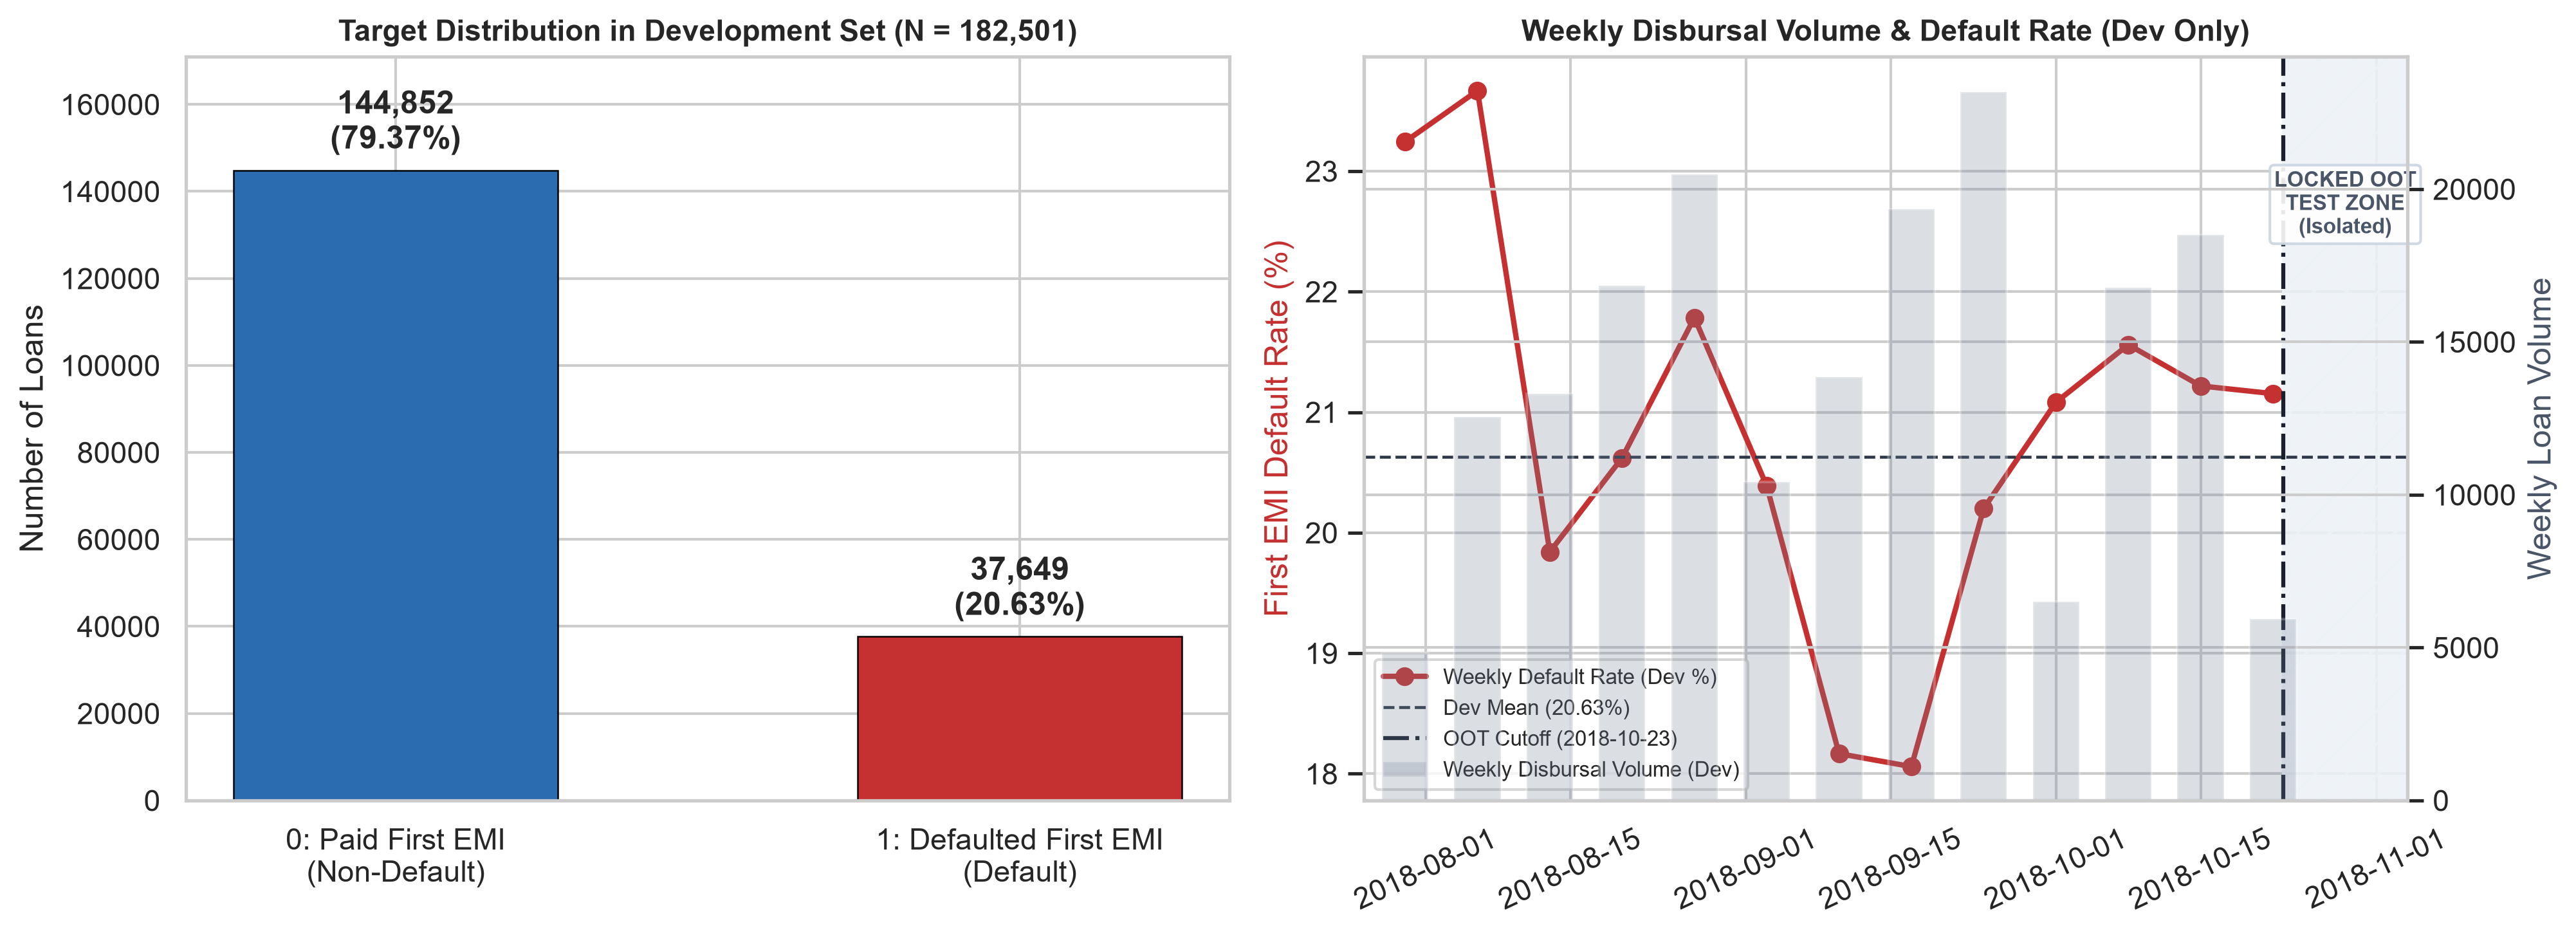
\includegraphics[width=0.95\textwidth]{figures/eda_01_target_and_splits.png}
  \caption{Development-set target distribution ($N = 182{,}501$, left) and weekly loan volume alongside default rate drift up to the October 23 Out-of-Time cutoff (right).}
  \label{fig:eda_target}
\end{figure}

Figure~\ref{fig:eda_bureau} demonstrates why the raw \texttt{PERFORM\_CNS.SCORE} field cannot be treated as a single continuous number. More than half of borrowers hold special status codes below $300$, whose default risk varies by reason code---from $17.6\%$ in Development ($18.6\%$ full corpus) for stale/inactive histories up to $24.1\%$ Dev ($25.6\%$ full corpus) for insufficient-history flags. Conversely, among scored borrowers ($300\text{--}890$), default risk exhibits a broadly upward trend across alphabetical risk grades \texttt{A}--\texttt{M}---rising from $12.0\%\text{--}16.5\%$ in Development ($13.1\%\text{--}17.3\%$ full corpus) for tiers \texttt{A}--\texttt{D} to $29.3\%$ Dev ($30.5\%$ full corpus) in tier \texttt{M}, with minor local inversions at grades \texttt{B}, \texttt{D}, and \texttt{J}.

\begin{figure}[htbp]
  \centering
  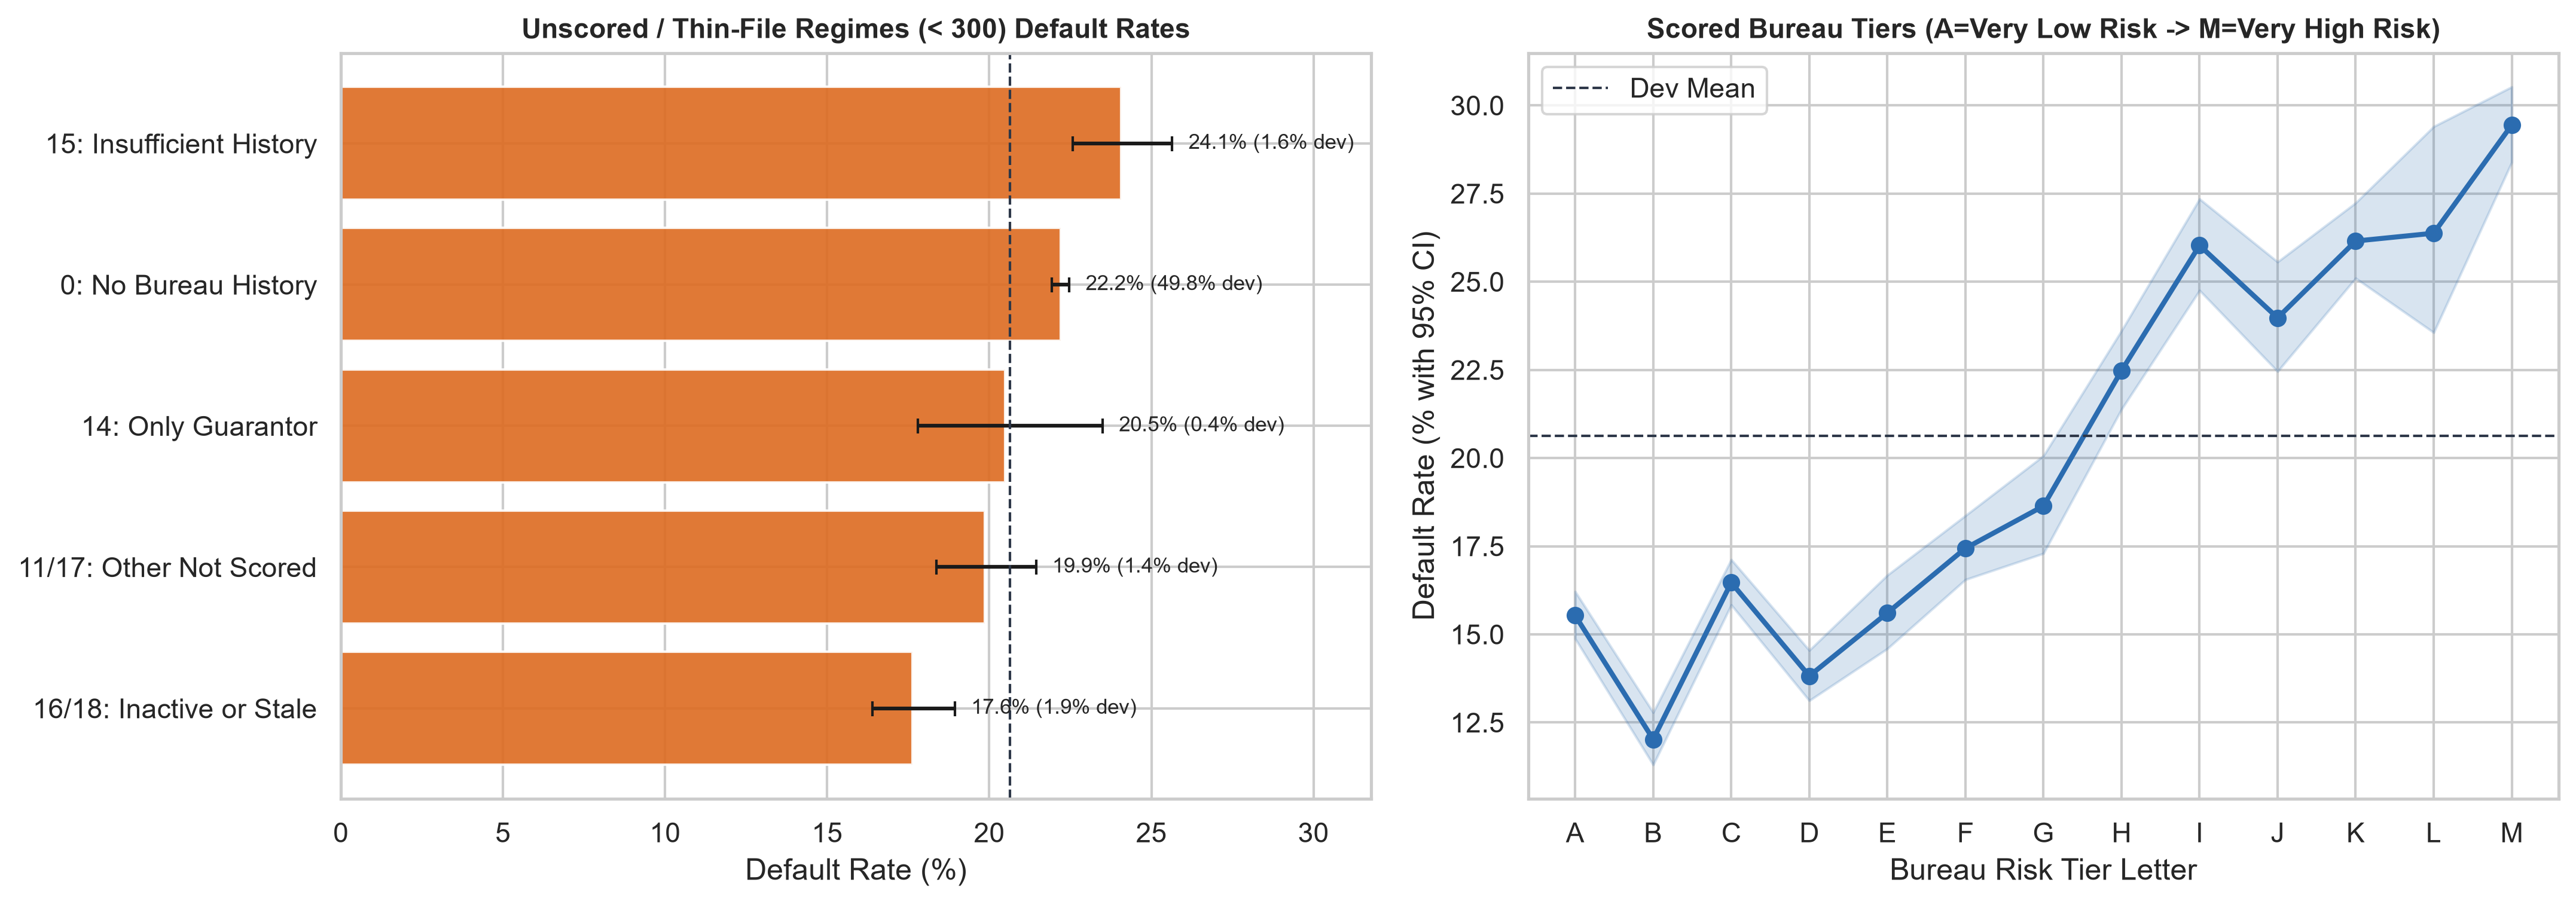
\includegraphics[width=0.95\textwidth]{figures/eda_04_bureau_regime_and_score_risk.png}
  \caption{Dual-regime credit bureau risk in the Development Set ($N = 182{,}501$): non-scored thin-file codes ($<300$, left) versus broad upward risk progression across scored tiers \texttt{A}--\texttt{M} (right).}
  \label{fig:eda_bureau}
\end{figure}

Further exploratory checks revealed three additional signals that guided feature design: (i) loan-to-value leverage (\texttt{ltv}) strongly stratifies default risk, nearly doubling from $13.1\%$ in the lowest decile to $25.8\%$ in the highest decile (and exceeding $29\%$ for high-LTV thin-file loans); (ii) \texttt{Self employed} borrowers default more frequently ($21.7\%$ on Dev) than \texttt{Salaried} ($19.4\%$) or missing-employment records ($20.0\%$); and (iii) ledger inconsistencies contain predictive risk signals, such as borrowers whose overdue accounts exceed active accounts ($27.5\%$ full-corpus default), current balances exceeding sanctioned limits ($24.3\%$), negative primary credit balances ($14.5\%$; $14.1\%$ combined primary/secondary), or gaps $>5$ percentage points between declared and computed LTV ($3.5\%$ of contracts).
